\documentclass[12pt,letterpaper,oneside,openany,spanish]{book}

\usepackage[spanish]{babel}
\usepackage[utf8]{inputenc}
\usepackage{siunitx} % Provides the \SI{}{} and \si{} command for typesetting SI units
\usepackage{graphicx} % Required for the inclusion of images
\usepackage{amsmath} % Required for some math elements 
\usepackage{hyperref}
\usepackage{amsmath}
\usepackage{listings}
\usepackage{courier}
\usepackage[margin=1.2in]{geometry}
\usepackage{changepage}
\usepackage{titlesec}
\usepackage{wrapfig}
\usepackage{colortbl}
\usepackage{booktabs}
\usepackage{multirow}
\usepackage{newtxtext,newtxmath}
\usepackage[utf8]{inputenc}
\usepackage[spanish]{babel}
\usepackage{graphicx}
\usepackage{amsmath} 
\usepackage{hyperref}
\usepackage[dvipsnames,table,xcdraw]{xcolor}
\usepackage{courier}
\usepackage{geometry}
\usepackage{changepage}
\usepackage{titlesec}
\usepackage{wrapfig}
\usepackage[version=4]{mhchem}
\usepackage{multirow}
\usepackage{siunitx}
\usepackage{tikz}
\usepackage{epigraph}
\usepackage{titlesec}
\usepackage{ragged2e}
\usepackage{multicol}
\usepackage{float}
\usepackage{pdfpages}
\usepackage{csquotes}
\usepackage{array}
\usepackage[shortlabels]{enumitem}
\usepackage{animate}
\usepackage{minitoc}

\definecolor{codegreen}{rgb}{0,0.6,0}
\definecolor{codegray}{rgb}{0.5,0.5,0.5}
\definecolor{codepurple}{rgb}{0.58,0,0.82}
\definecolor{backcolour}{rgb}{0.95,0.95,0.92}

\lstdefinestyle{mystyle}{
    backgroundcolor=\color{backcolour},   
    commentstyle=\color{codegreen},
    keywordstyle=\color{magenta},
    numberstyle=\tiny\color{codegray},
    stringstyle=\color{codepurple},
    basicstyle=\ttfamily\footnotesize,
    breakatwhitespace=false,         
    captionpos=b,                    
    keepspaces=true,                 
    numbers=left,                    
    numbersep=5pt,                  
    showspaces=false,                
    showstringspaces=false,
    showtabs=false,                  
    tabsize=2
}
\lstset{language=Python, 
        basicstyle=\ttfamily\small, 
        keywordstyle=\color{keywords},
        commentstyle=\color{comments},
        stringstyle=\color{red},
        showstringspaces=false,
        identifierstyle=\color{codepurple},
        keywords=[2]{pow},
        keywordstyle=[2]{\color{orange}},
}

\lstset{style=mystyle}

\setlength\parindent{0pt} % Removes all indentation from paragraphs

\renewcommand{\labelenumi}{\alph{enumi}.} % Make numbering in the enumerate environment by letter rather than number (e.g. section 6)

\begin{document}
   

\newcommand{\titulo}{Informes sobre prácticas demostrativas}
\newcommand{\nombreestudiante}{Víctor Mira Ramírez}
\newcommand{\nombredirector}{Ángel Ávila Freire}
\newcommand{\fecha}{\date{Febrero 2023}}  % Definir solo el año de presentación


\pagebreak

\renewcommand{\listtablename}{Índice de tablas} 
\renewcommand{\tablename}{Tabla} 

\begin{titlepage}
	\centering
	
\includegraphics[width=65mm]{Fotos/logoUA.png}\par
	\vspace{1cm}
	{\LARGE\bfseries \titulo \par}
	\vfill
	{\large Breves informes de laboratorio acerca de \\ 
	dos prácticas demostrativas propuestas\par
	\vfill
	Estudiante:\par\vspace{2mm}
	\nombreestudiante\par
	\vfill
	Profesor:\par\vspace{2mm}
    \nombredirector
    \vfill
    Universidad de Alicante\par
    Facultad de Ciencias: Departamento de Física Aplicada\par
    Técnicas experimentales I\par
	\fecha\par}
\end{titlepage}

\pagebreak
\tableofcontents
\pagebreak

% PRÁCTICA 1
\pagenumbering{arabic}
\setcounter{page}{4}
    \chapter[TD4. Variación de la presión]{TD4. Variación de la presión}
    \thispagestyle{empty}
    \vspace{1cm}
    \begin{figure}[h]
        \centering
        \hspace*{-0.2cm}
        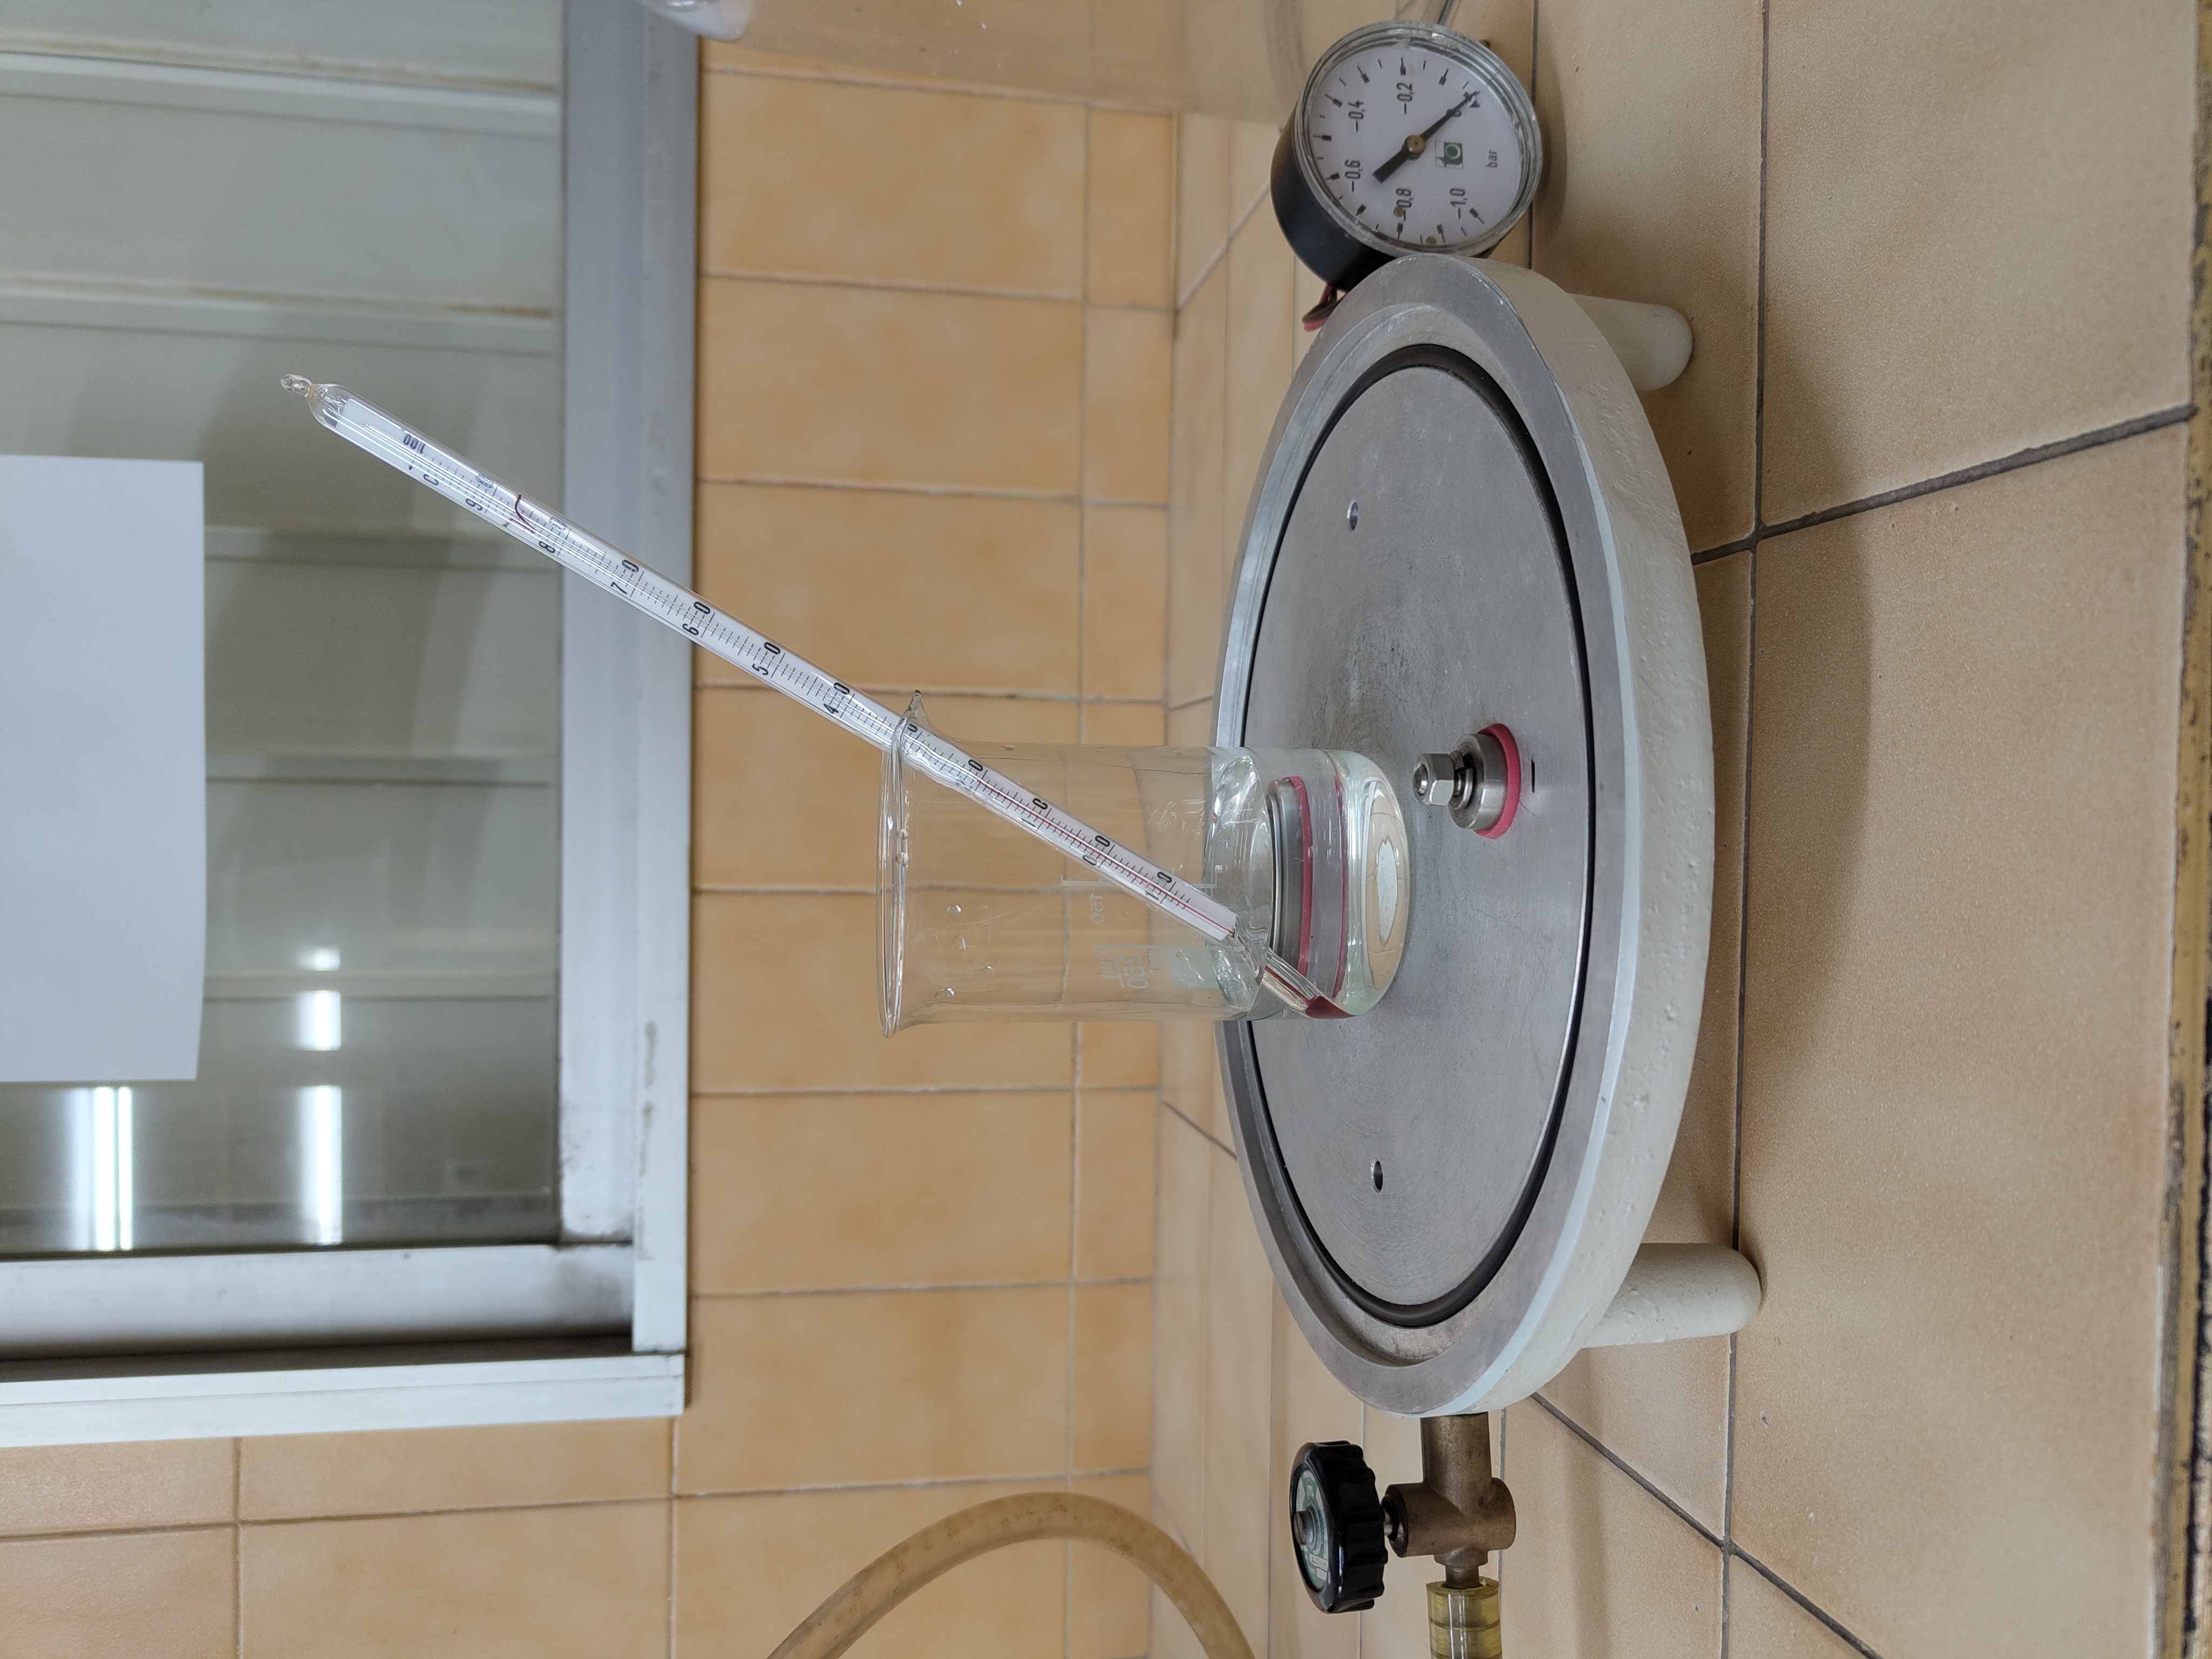
\includegraphics[angle=270,origin=c,width=.48\textwidth]{Fotos/Vacío/portada 2.jpg}\hfill
        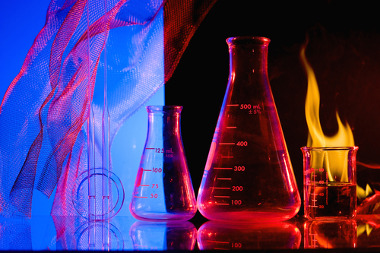
\includegraphics[angle=270,origin=c,width=.48\textwidth]{Fotos/Vacío/portada.jpg}
        \hspace*{-0.4cm}
    \end{figure}
\include{vacío}

% PRÁCTICA 2
\chapter[TD2. Pajarillo bebedor]{TD2. Pajarillo bebedor}
\thispagestyle{empty}
\vspace{1cm}
\begin{figure}[h]
    \centering
    \hspace*{-0.2cm}
    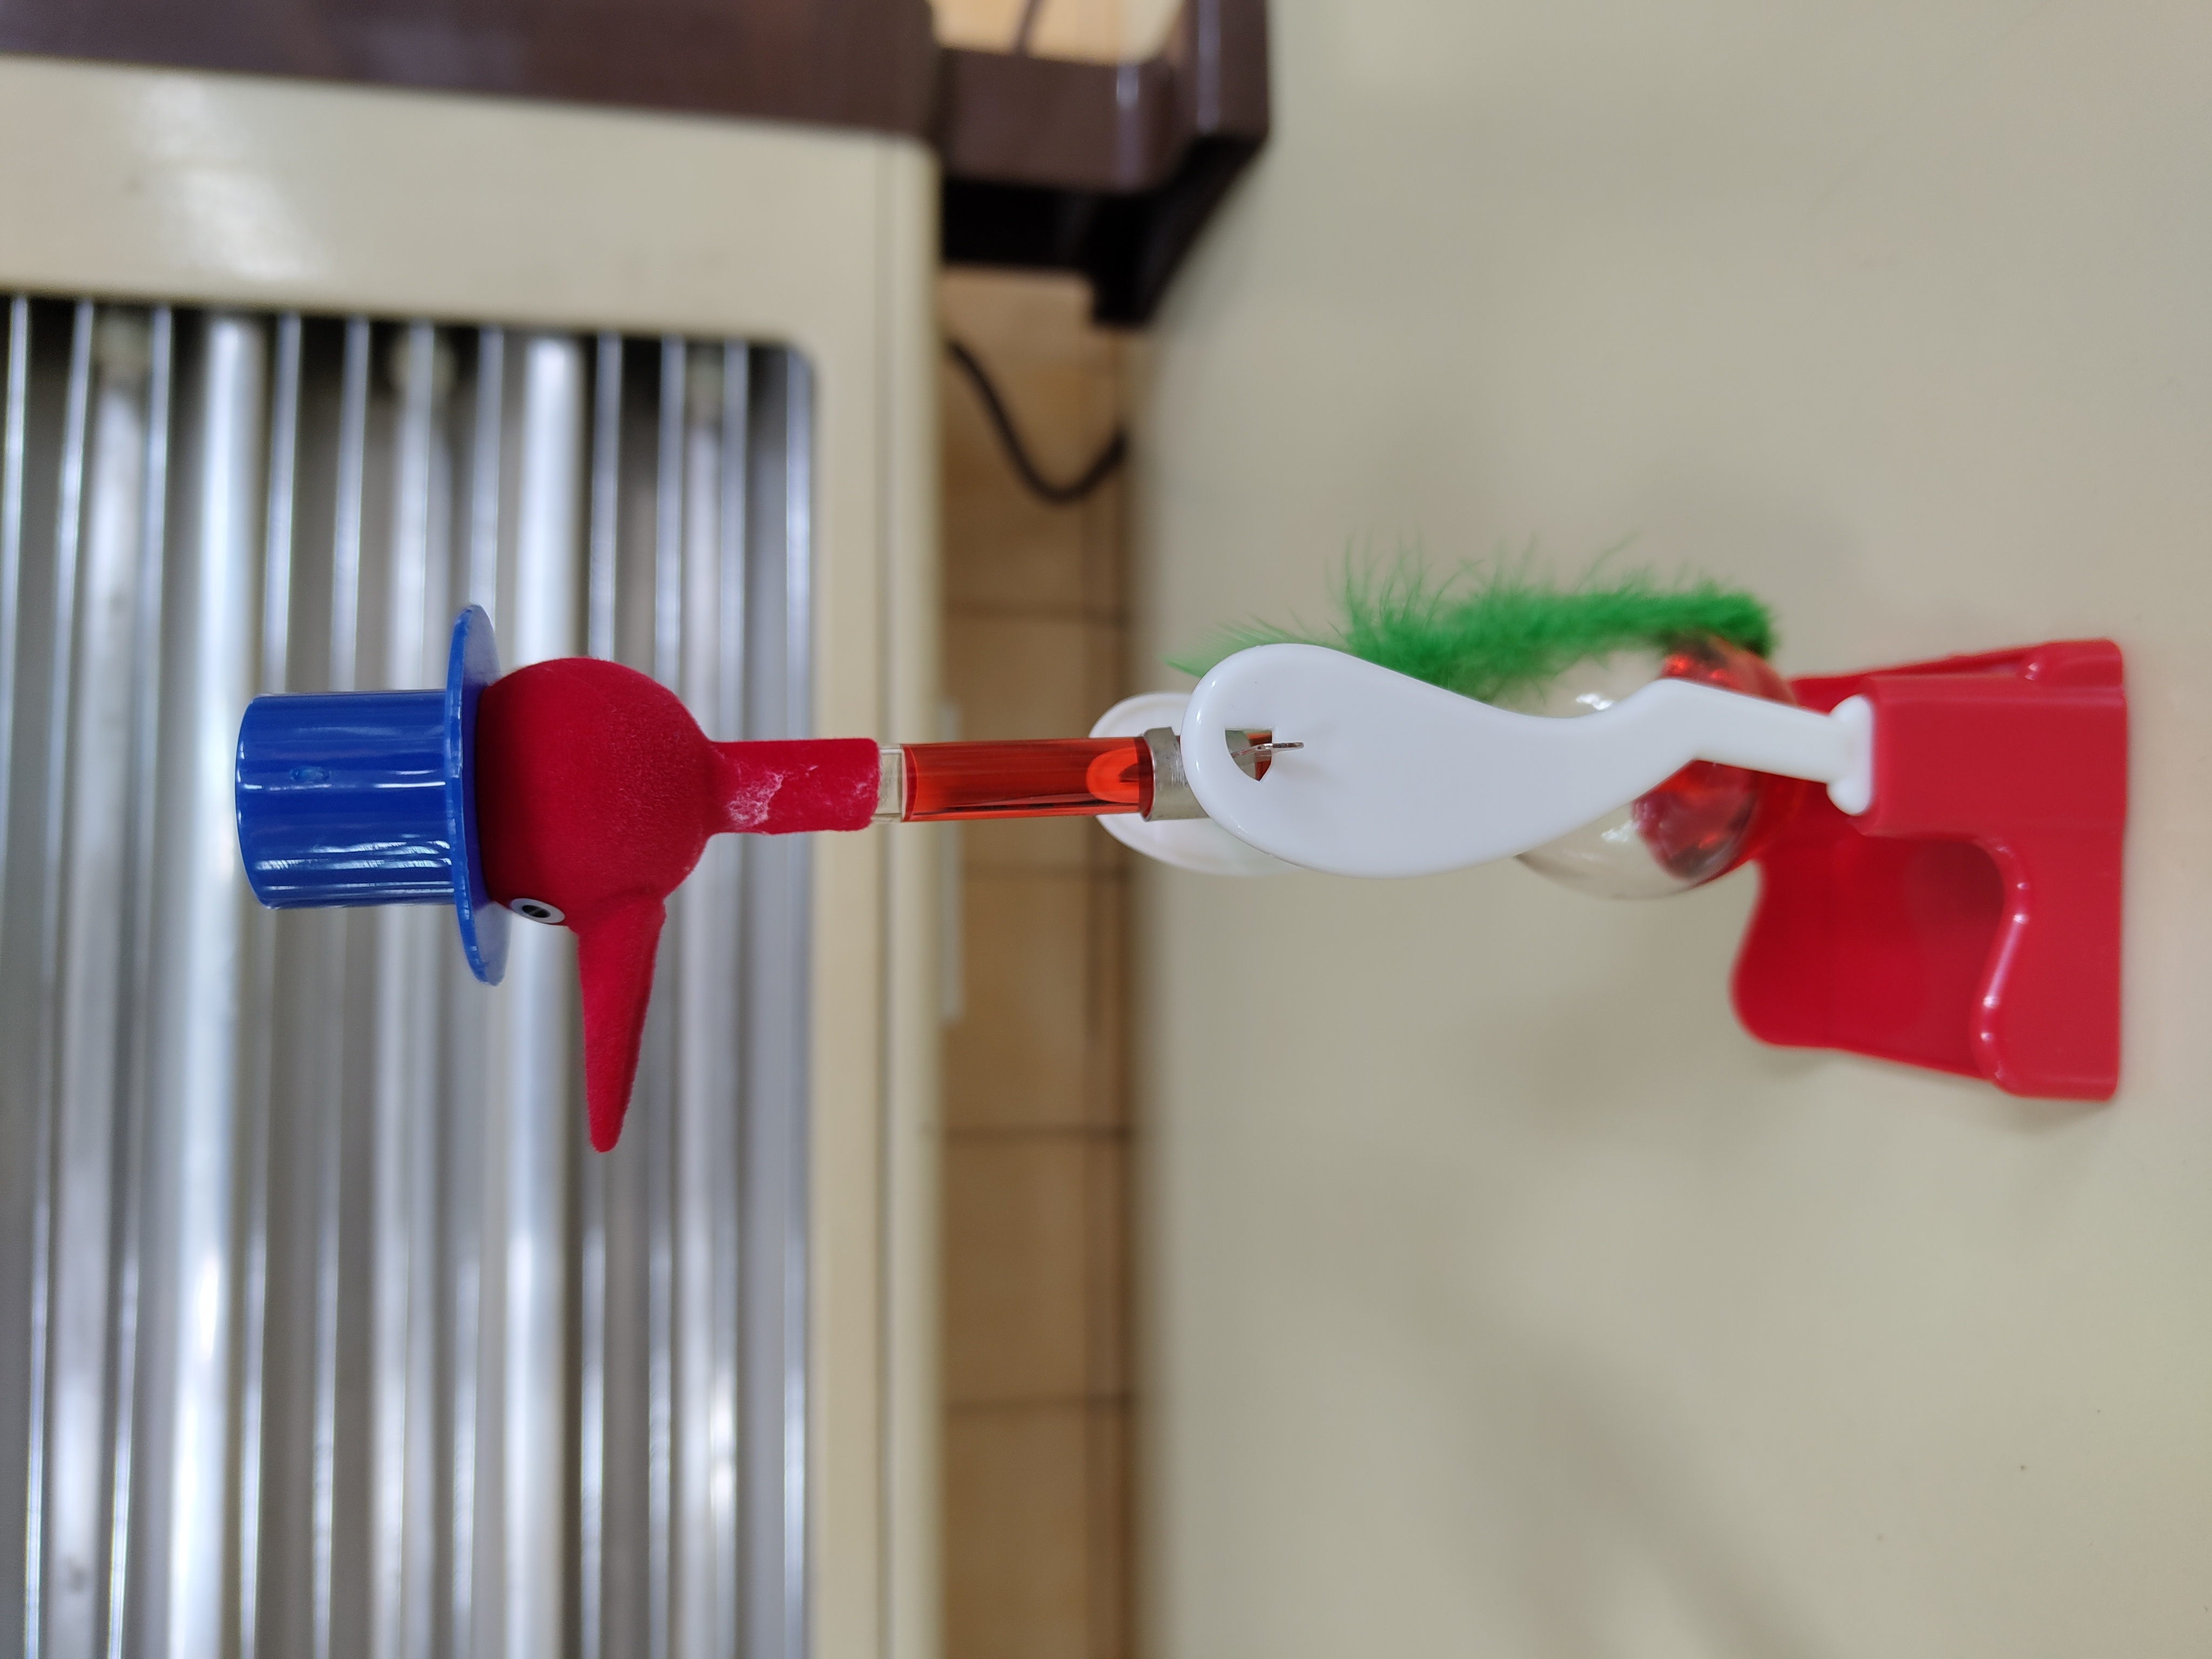
\includegraphics[width=.8\textwidth,angle=270]{Fotos/Pajarillo/Portada.jpg}
    \hspace*{-0.4cm}
    \end{figure}                                      
\section{Introducción}
    \subsection{Objetivos}
        En este breve informe descubriremos y analizaremos el comportamiento de el famoso juguete conocido como \textit{El pájaro bebedor} desde el punto de vista de la termodinámica. Usaremos nuestros conocimientos, además de los contenidos vistos en las clases de laboratorio, para describir el funcionamiento de este artilugio.
    \subsection{Descripción de la experiencia}
        La experiencia de laboratorio es bastante simple, tendremos dos elementos indispensables, el cuerpo que se asemeja a un pájaro, un vaso de agua, y en algunas ocasiones, un calefactor (más adelante describiremos en qué ocasiones específicamente).\\ \\Podemos observar que el juguete en sí está compuesto por dos elementos, un soporte con un eje y sobre dicho eje, un tubo libre de girar. Dentro del tubo (que está decorado para que se asemeje a un ave) vemos un líquido tintado de rojo. Observamos además que el tubo se engrosa en la parte inferior y nos deja ver que hay un segundo tubo dentro de él.\\ \\La experiencia realmente comienza cuando ponemos el juguete al lado del vaso de agua, y inclinamos el tubo hasta que el "pico" del pájaro toca la superficie del vaso de agua. Inmediatamente después el tubo oscila alrededor de la posición vertical, solo que cada vez con más lentitud. Dichas oscilaciones se enlentecen pero crecen en amplitud hasta que el "pico" del pájaro vuelve a tocar la superficie del agua y entramos en un ciclo que no cesa.\\ \\Cabe nombrar que si la temperatura ambiente es inferior a unos $20$ $\si{\celsius}$, será necesario el uso de un calefactor que mantenga dicha temperatura alrededor del juguete.\\
        \begin{figure}[h]\label{fig:horizontal}
            \centering
            \animategraphics[autoplay,loop,width=8cm,controls=all]{30}{Fotos/Pajarillo/gif/target-}{0}{199}
            \caption{Experiencia en acción}
        \end{figure}
\clearpage
\section{Propuesta de Hipótesis}
    A primera vista el juguete parece casi imposible, vemos un objeto que tras un aporte de energía externo (bajarlo hasta que toque el agua), continúa moviéndose desafiando toda lógica. ¿Acaso ha resuelto este pajarillo los problemas energéticos de toda la humanidad?\\ \\Obviamente no es el caso así que es natural preguntarse qué es lo que hace que el pajarito se mueva sin cesar. La primera idea que se le viene a uno a la cabeza es que cierto proceso termodinámico en el interior del cuerpo del ave es el causante del movimiento. Además la necesidad de una temperatura ambiente mayor a un umbral, y la opacidad de la cabeza del juguete nos da una pista de lo que puede estar sucediendo.\\ \\Entonces, ¿Cuál es el proceso termodinámico que estamos presenciando? El cambio de fase. Las fases de una sustancia son los distintos estados homogéneos que puede alcanzar con la variación de sus variables termodinámicas. Las fases de este líquido que están sucediéndose son la gaseosa y la líquida.\\ \\Una vez empezado el movimiento, cuando el pajarito vuelve a la posición de equilibrio pero oscila alrededor de esta, la sustancia del interior se encuentra en fase gaseosa dentro de la cabeza del pajarito, pero en fase líquida en la "cola". El líquido asciende poco a poco a causa de la diferencia de presiones entre la cabeza y la cola, subiendo el centro de gravedad del pajarito y haciendo que cada vez oscile más y más hasta llegar a ponerse horizontal. En ese momento, la superficie del líquido rebasa el segundo tubo como podemos ver en la figura \ref{fig:horizontal}, lo cual hace que el gas se pueda introducir dentro del tubo y hacer caer todo el líquido que había ascendido. Esto, vuelve a cambiar el centro de masas, solo que esta vez lo hace bajar, haciendo que el pajarito vuelva a la posición de equilibrio.\\ \\Y es que, cuando el pico del pájaro toca la superficie del agua, el gas que hay en la cabeza del pájaro se condensa, lo cual produce la diferencia de presiones que hace ascender el líquido. Cuando el pájaro ya no toca el agua, si no que está a temperatura ambiente, parte del líquido se evapora, haciendo que el movimiento se repita.
\section{Comprobación y discusión}
    Lo más destacable de la experiencia es ver como un artilugio que parece tener energía infinita, no es más que un truco termodinámico. Al final, lo que mantiene el pajarito en movimiento no es más que la diferencia de temperatura entre el ambiente y el agua. Y es que cuando sacamos agua del grifo, esta suele estar a una temperatura algo menor a la ambiente. Es por eso que cuando el agua, el pajarito y el ambiente estén a la misma temperatura, el pajarito acabará por pararse. Por eso es necesario el calefactor en algunos casos, cuando el agua se atempera con el ambiente, si subimos la temperatura ambiente por medio de un calefactor, volveremos a generar esta diferencia de temperaturas con el agua y permitiremos el movimiento.
\section{Sugerencias experimentales}
    Realmente el experimento es tan sencillo que no es fácil encontrar puntos de mejora obvios. Sin embargo voy a proponer algunos puntos que pienso que podrían mejorar la experiencia en su conjunto. Me centro específicamente en el juguete en sí, que tal vez podría tener un mayor tamaño para facilitar ver qué sucede en su interior. Con este mismo objetivo, pienso que una mayor visibilidad del interior de la cabeza del pajarillo facilitaría la comprensión del funcionamiento del mismo. Sin embargo, esto iría a expensas de su apariencia de ave además de la "magia" de dilucidar el funcionamiento del artilugio sin destriparlo tanto.

\end{document}
